\documentclass{article}
\usepackage[utf8]{inputenc}
\usepackage[margin=0.4in]{geometry}


\title{Computer Networks HW 3}
\author{Shane Cincotta }
\date{April 8, 2020}

\usepackage{natbib}
\usepackage{graphicx}

\begin{document}

\maketitle

\section*{Chapter 3, Review Question 3}
The source port now becomes \textit{y} and the destination port becomes \textit{x}.\\

\section*{Chapter 3, Review Question 6}
Yes it is possible.  The biggest hurdles include having mechanisms for resending lost packets, checking for corrupted packets, sending acknowledgements, etc.  This can be done if the mechanisms are built into the program itself.\\

\section*{Chapter 3, Review Question 7}
Yes, both of these segments be directed to the same socket at Host C. Although the destination ports of hosts A and B are the same, they have different source addresses in the form of an IP address.\\

\section*{Chapter 3, Review Question 9}
The purpose for sequence numbers was to let the receiver know whether the incoming packet was a new packet or a retransmission.\\

\section*{Chapter 3, Review Question 10}
Timers were introduced to act as a timeout to trigger retransmission.  After a certain amount of time has passed without receiving an ACK, the packet is assumed lost and will be sent again,\\

\section*{Chapter 3, Problem 2}
% What are the source and destination port values in the segments flowing from the server back to the clients’ processes? What are the IP addresses in the network-layer datagrams carrying the transport-layer segments?
From server to host A:\\
\newline Source port = 80, destination port = 26145.\\
Source IP = B, destination IP = A.\\
\newline From server B to host C (Left process):\\
\newline Left process: Source port = 80, destination port = 7532.\\
Source IP = B, destination IP = C.\\
\newline From server B to host C (Right process):\\
\newline Source port = 80, destination port = 26145.\\
Source IP = B, destination IP = C.\\
\clearpage

\section*{Chapter 3, Problem 3}
$01010011 = 83$\\
$01100110 = 102$\\
$01110100 = 116$\\
\newline $83 + 102 + 116 = 301$\\
$301 = 100101101$\\
\newline Account for carry bit:\\
$100101101 = 00101110$\\
\newline 1s compliment of $00101110 = 11010001$\\
\newline UDP takes the 1s compliment instead of just the sum because some ISAs use little endian and some use big endian notation.  Computing the checksum on two machines which use different notation could lead to different results.  Using 1s compliment ensures that the checksum is the same regardless of which notation the ISA uses.\\
\newline To detect errors, the receiver will add all the bytessnd look at the sum.  If the sum contains all 1s, there is no error, if there is at least one 0, there are errors.  All one-bit errors will be detected but two-bit errors cannot be detcted.\\

\section*{Chapter 3, Problem 5}
No, its possible that the  calculated checksum matches the value in the checksum field, but still contains errors.  For example, if when we add two 16-bit numbers, its possible that the the corresponding bits are flipped to 0 or 1.  In this case, the sum will be the same and thus the 1s compliment will be equal to the checksum, even though there are errors they go undetected.\\

\section*{Chapter 3, Problem 8}
\begin{figure}[h!]
\centering
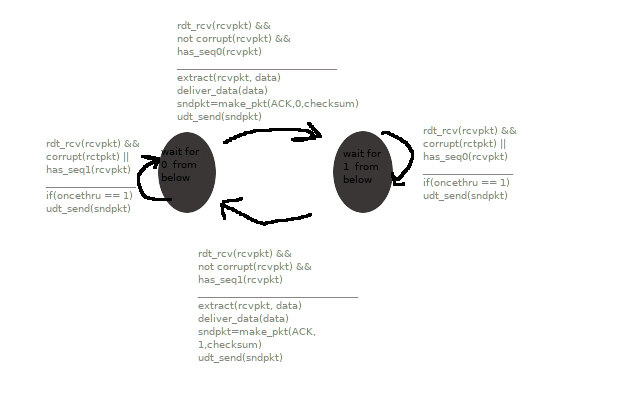
\includegraphics[scale=0.45]{P8.png}
\caption{FSM for the receiver side}
\end{figure}
\clearpage

\section*{Chapter 3, Problem 9}
\begin{figure}[h!]
\centering
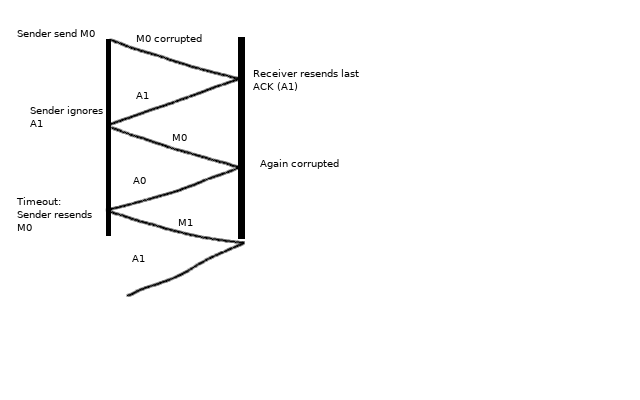
\includegraphics[scale=0.5]{P9a.png}
\caption{Corrupted data packets}
\end{figure}

\begin{figure}[h!]
\centering
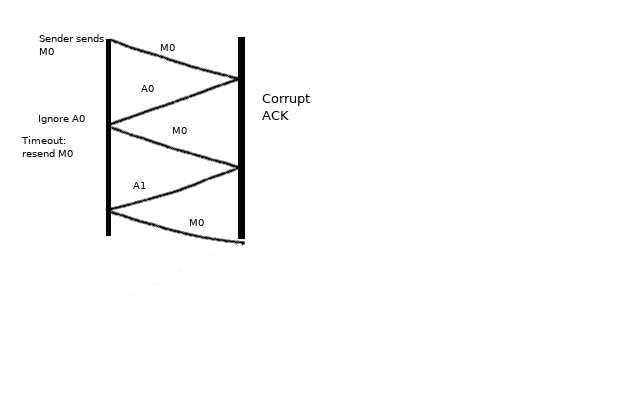
\includegraphics[scale=0.5]{P9b.png}
\caption{Corrupted ACK}
\end{figure}
\clearpage
\section*{Chapter 3, Problem 13}

\begin{figure}[h!]
\centering
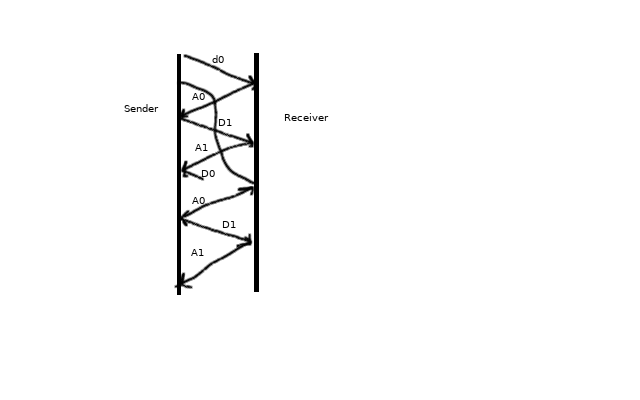
\includegraphics[scale=0.5]{P13.png}
\caption{Reordering messages}
\end{figure}
First, the sender sends the data D0 and waits for the acknowledgement A0 from the receiver.  The sender does not receive A0 in time, and assume it is lost.  The sender then resends D0.  When the sender receives A0, it sends D1.  The sender receives A1, then receives A0 for the retransmitted D0.  The receiver has gotten the old version of D0 and acknowledges it, so the sender again sends the data D1 and receiver sends A1 for D1 to the sender.  Thus D0 is being replaced by an older version, as improper data is being sent.\\

\section*{Chapter 3, Problem 15}
$D_{trans} = \frac{L}{R} = \frac{1500*8}{10^{9}} = 0.012$ milliseconds.\\
\newline Channel utilization = $N*\frac{\frac{L}{R}}{\frac{L}{R}+RTT}$\\
\newline $0.98 = WS*\frac{\frac{L}{R}}{\frac{L}{R}+RTT}$\\
\newline $WS = 2450.98$\\
\newline The window size needs to be about 2451.\\

\section*{Chapter 3, Problem 22}
\subsection*{a}
If all the packets up to k-1 have been ACKd, the sender's window range will be [k, k+N-1].  It begins at k because k-1 have been ACKd, so k is the start of the next sequence number.  The maximum is k+N-1.\\
\newline If the sender doesn't receive any AKCs, the range will be [k-N, k-1], because it has to resend the window.\\
\newline Thus the sets of possible sequence numbers inside the sender's window are in the range [k-N, k]\\

\subsection*{b}
The sender will never send an ACK less than k-N-1 back, and never send a value greater than k-1.  Thus the range is [k-N-1, k-1].\\
\clearpage

\section*{Chapter 3, Problem 23}
The sequence number space must be at least twice as large as the window size.\\

\section*{Chapter 3, Problem 24}
\subsection*{a}
True.\\
\newline For example, a sender is waiting for the ACKs to a set of packets it sent.  The sender timesout and resends the packets.  It then receives the ACK for the resent packets and moves the window.  Then, after the window is moved, the ACKs that timed out are received, these ACK numbers will fall outside the current window.\\
\subsection*{b}
True.\\
\newline For example, a sender is waiting for the ACKs to a set of packets it sent.  The sender timesout and resends the packets.  It then receives the ACK for the resent packets and moves the window.  Then, after the window is moved, the ACKs that timed out are received, these ACK numbers will fall outside the current window.\\

\subsection*{c}
True.\\
\newline  In alternating-bit protocol, the sequence number fluctuates between 0 and 1, which coincides with a window size of 1.\\

\subsection*{d}
True.\\
\newline The packet is referred as a single packet within the window.  The ACK is treated as an ordinary ACK.\\

\end{document}